76. $y=\cfrac{x^3-x}{|x|}=\cfrac{x(x^2-1)}{|x|}=\begin{cases} x^2-1,\ x>0,\\ 1-x^2,\ x<0.\end{cases}$
$$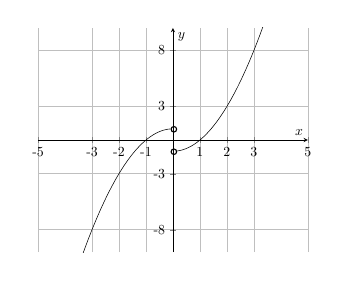
\begin{tikzpicture}[scale=0.5]
\begin{axis}[
    axis lines = middle,
    grid=major,
    legend pos={south west},
    xlabel = {$x$},
    %xlabel style={below right},
    ylabel = {$y$},
    ymin=-10,
    ymax=10,
    xmin=-5,
    xmax=5,
    xtick={-5,-3,-2,-1,1,2,3,5},
    xticklabels={-5,-3,-2,-1,1,2,3,5},
    ytick={-8,8,3,-3},
    yticklabels={-8,8,3,-3},
                  ]
	\addplot[domain=-5:-0.1, samples=100, color=black] {(x*x*x-x)/abs(x)};
    \addplot[domain=0.1:5, samples=100, color=black] {(x*x*x-x)/abs(x)};
        %\addplot[domain=2.01:6, samples=100, color=black] {2/(2-x)};
   % \addplot[domain=-3:3, samples=100, color=black] {-x};
     %\addlegendentry{$\text{Рис. 1}$};
\end{axis}
\draw (3.45,3.12) circle (2pt);
\draw (3.45,2.55) circle (2pt);
\end{tikzpicture}$$
